\documentclass[
	11pt, % Set the default font size, options include: 8pt, 9pt, 10pt, 11pt, 12pt, 14pt, 17pt, 20pt
	%t, % Uncomment to vertically align all slide content to the top of the slide, rather than the default centered
	aspectratio=169, % Uncomment to set the aspect ratio to a 16:9 ratio which matches the aspect ratio of 1080p and 4K screens and projectors
]{beamer}

\graphicspath{{plots/}{images/}} % Specifies where to look for included images (trailing slash required)
\usepackage{booktabs} % Allows the use of \toprule, \midrule and \bottomrule for better rules in tables
\usetheme{Madrid} % A good all-around theme
\usefonttheme{default} % Typeset using the default sans serif font
\usepackage{palatino} % Use the Palatino font for serif text
\usepackage[default]{opensans} % Use the Open Sans font for sans serif text
\useinnertheme{circles}
\title[Universality]{10K Feet View of Universality} % The short title in the optional parameter appears at the bottom of every slide, the full title in the main parameter is only on the title page
\author[Aditya \and Dhano \and Sapna]{Aditya Mehta \and Dhananjay Raman \and Sapna} % Presenter name(s), the optional parameter can contain a shortened version to appear on the bottom of every slide, while the main parameter will appear on the title slide
\institute[IITB]{Indian Institute of Technology, Bombay} % Your institution, the optional parameter can be used for the institution shorthand and will appear on the bottom of every slide after author names, while the required parameter is used on the title slide and can include your email address or additional information on separate lines
\date[October 4, 2023]{PH 567 Presentation \\ October 4, 2023} % Presentation date or conference/meeting name, the optional parameter can contain a shortened version to appear on the bottom of every slide, while the required parameter value is output to the title slide
\begin{document}

%----------------------------------------------------------------------------------------
%	TITLE SLIDE
%----------------------------------------------------------------------------------------

\begin{frame}
	\titlepage % Output the title slide, automatically created using the text entered in the PRESENTATION INFORMATION block above
\end{frame}

%----------------------------------------------------------------------------------------
%	TABLE OF CONTENTS SLIDE
%----------------------------------------------------------------------------------------

% The table of contents outputs the sections and subsections that appear in your presentation, specified with the standard \section and \subsection commands. You may either display all sections and subsections on one slide with \tableofcontents, or display each section at a time on subsequent slides with \tableofcontents[pausesections]. The latter is useful if you want to step through each section and mention what you will discuss.

\begin{frame}
	\frametitle{Today's Topics} % Slide title, remove this command for no title
	
	\tableofcontents % Output the table of contents (all sections on one slide)
	%\tableofcontents[pausesections] % Output the table of contents (break sections up across separate slides)
\end{frame}

%----------------------------------------------------------------------------------------
%	PRESENTATION BODY SLIDES
%----------------------------------------------------------------------------------------

\section{The Theory} % Sections are added in order to organize your presentation into discrete blocks, all sections and subsections are automatically output to the table of contents as an overview of the talk but NOT output in the presentation as separate slides

%------------------------------------------------

\subsection{What is Universality?}

\begin{frame}
	\frametitle{What is Universality?}
	
	\begin{itemize}
        \item Universality is the observation that there are properties for a large class of systems that are independent of the dynamical details of the system
    \end{itemize}

\end{frame}

%------------------------------------------------

\subsection{The Tools}

\begin{frame}
	\frametitle{The Tools}
	There are a few properties that we can use to compare and contrast between different systems: \pause
    \begin{itemize}
        \item Bifurcation Points \pause
        \item Bifurcation Diagrams \pause
        \item Lyapunov Exponents
    \end{itemize}

\end{frame}

%------------------------------------------------

\begin{frame}
	\frametitle{Bifurcation Points}
    \begin{itemize}
        \item A bifurcation point is a point in the parameter space of a system at which a bifurcation occurs. \pause
        \item At a bifurcation point, a small change of the parameter value of the system may cause a large change in the number or stability (or structural form) of the equilibrium points of the system, or the emergence of limit cycles (oscillations), tori (higher-dimensional analogs of limit cycles), or chaos from an attracting orbit. \pause
        \item The bifurcation point itself does not represent any dynamical change of the system, but rather a \textcolor{red}{qualitative} change of its \textcolor{blue}{behavior} as one or more parameters crosses a \textcolor{teal}{critical threshold}.
    \end{itemize}
\end{frame}

%------------------------------------------------

\begin{frame}
	\frametitle{Bifurcation Diagram}
    \begin{itemize}
        \item A bifurcation diagram shows the values visited or approached asymptotically (fixed points, periodic orbits, or chaotic attractors) of a system as a function of a bifurcation parameter in the system. \pause
        \item For a one dimensional map the bifurcation parameter r is shown on the horizontal axis of the plot and the vertical axis shows the set of values of the logistic function visited asymptotically from almost all initial conditions.
    \end{itemize}
\end{frame}

%------------------------------------------------

\begin{frame}
	\frametitle{Example Bifurcation Diagram}
    \begin{figure}
        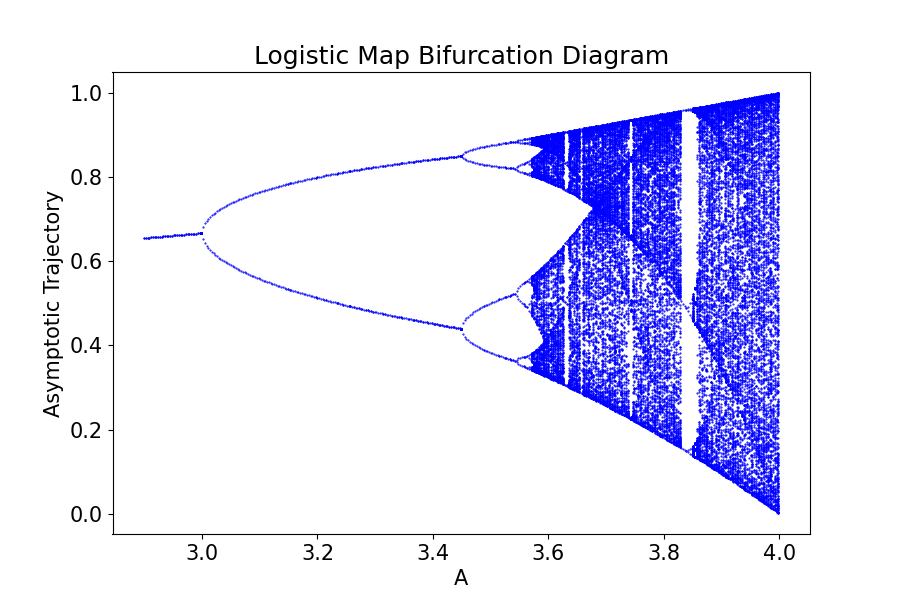
\includegraphics[width=0.6\linewidth]{logistic_bifurcation_diagram.png}
    \end{figure}
\end{frame}

%------------------------------------------------

\begin{frame}
	\frametitle{Lyapunov Exponents}
    \begin{itemize}
        \item Lyapunov exponents are used to quantify the rate of separation of infinitesimally close trajectories. \pause
        \item Two trajectories in phase space with initial separation vector $\delta_0$ diverge at a rate given by 
        \begin{equation}
            \delta_n = \delta_0 e^{\lambda n}
        \end{equation}
        where $\lambda$ is the Lyapunov exponent and $n$ is the number of iterations. \pause
        \item The Lyapunov exponent is \textcolor{red}{positive} for chaotic systems, \textcolor{blue}{zero} for non-chaotic systems, and \textcolor{teal}{negative} for systems that converge to fixed points.
    \end{itemize}
\end{frame}

%------------------------------------------------

\begin{frame}
	\frametitle{Lyapunov Exponents}
    \begin{itemize}
        \item For a one dimensional map $x_{n+1} = f(x_n)$, the Lyapunov exponent is given by
        \begin{equation}
            \lambda = \lim_{n \to \infty} \frac{1}{n} \sum_{i=0}^{n-1} \ln \left| f'(x_i) \right|
        \end{equation}
        where $f$ is the map and $x_i$ is the $i$th iterate of the map. \pause
        \item Typically, the lyapunov exponent is zero at the bifurcation points, and highly negative (Read: $-\infty$) at the superstable points.
    \end{itemize}
\end{frame}

%------------------------------------------------

\begin{frame}
	\frametitle{Example Lyapunov Exponent Plot}
    \begin{figure}
        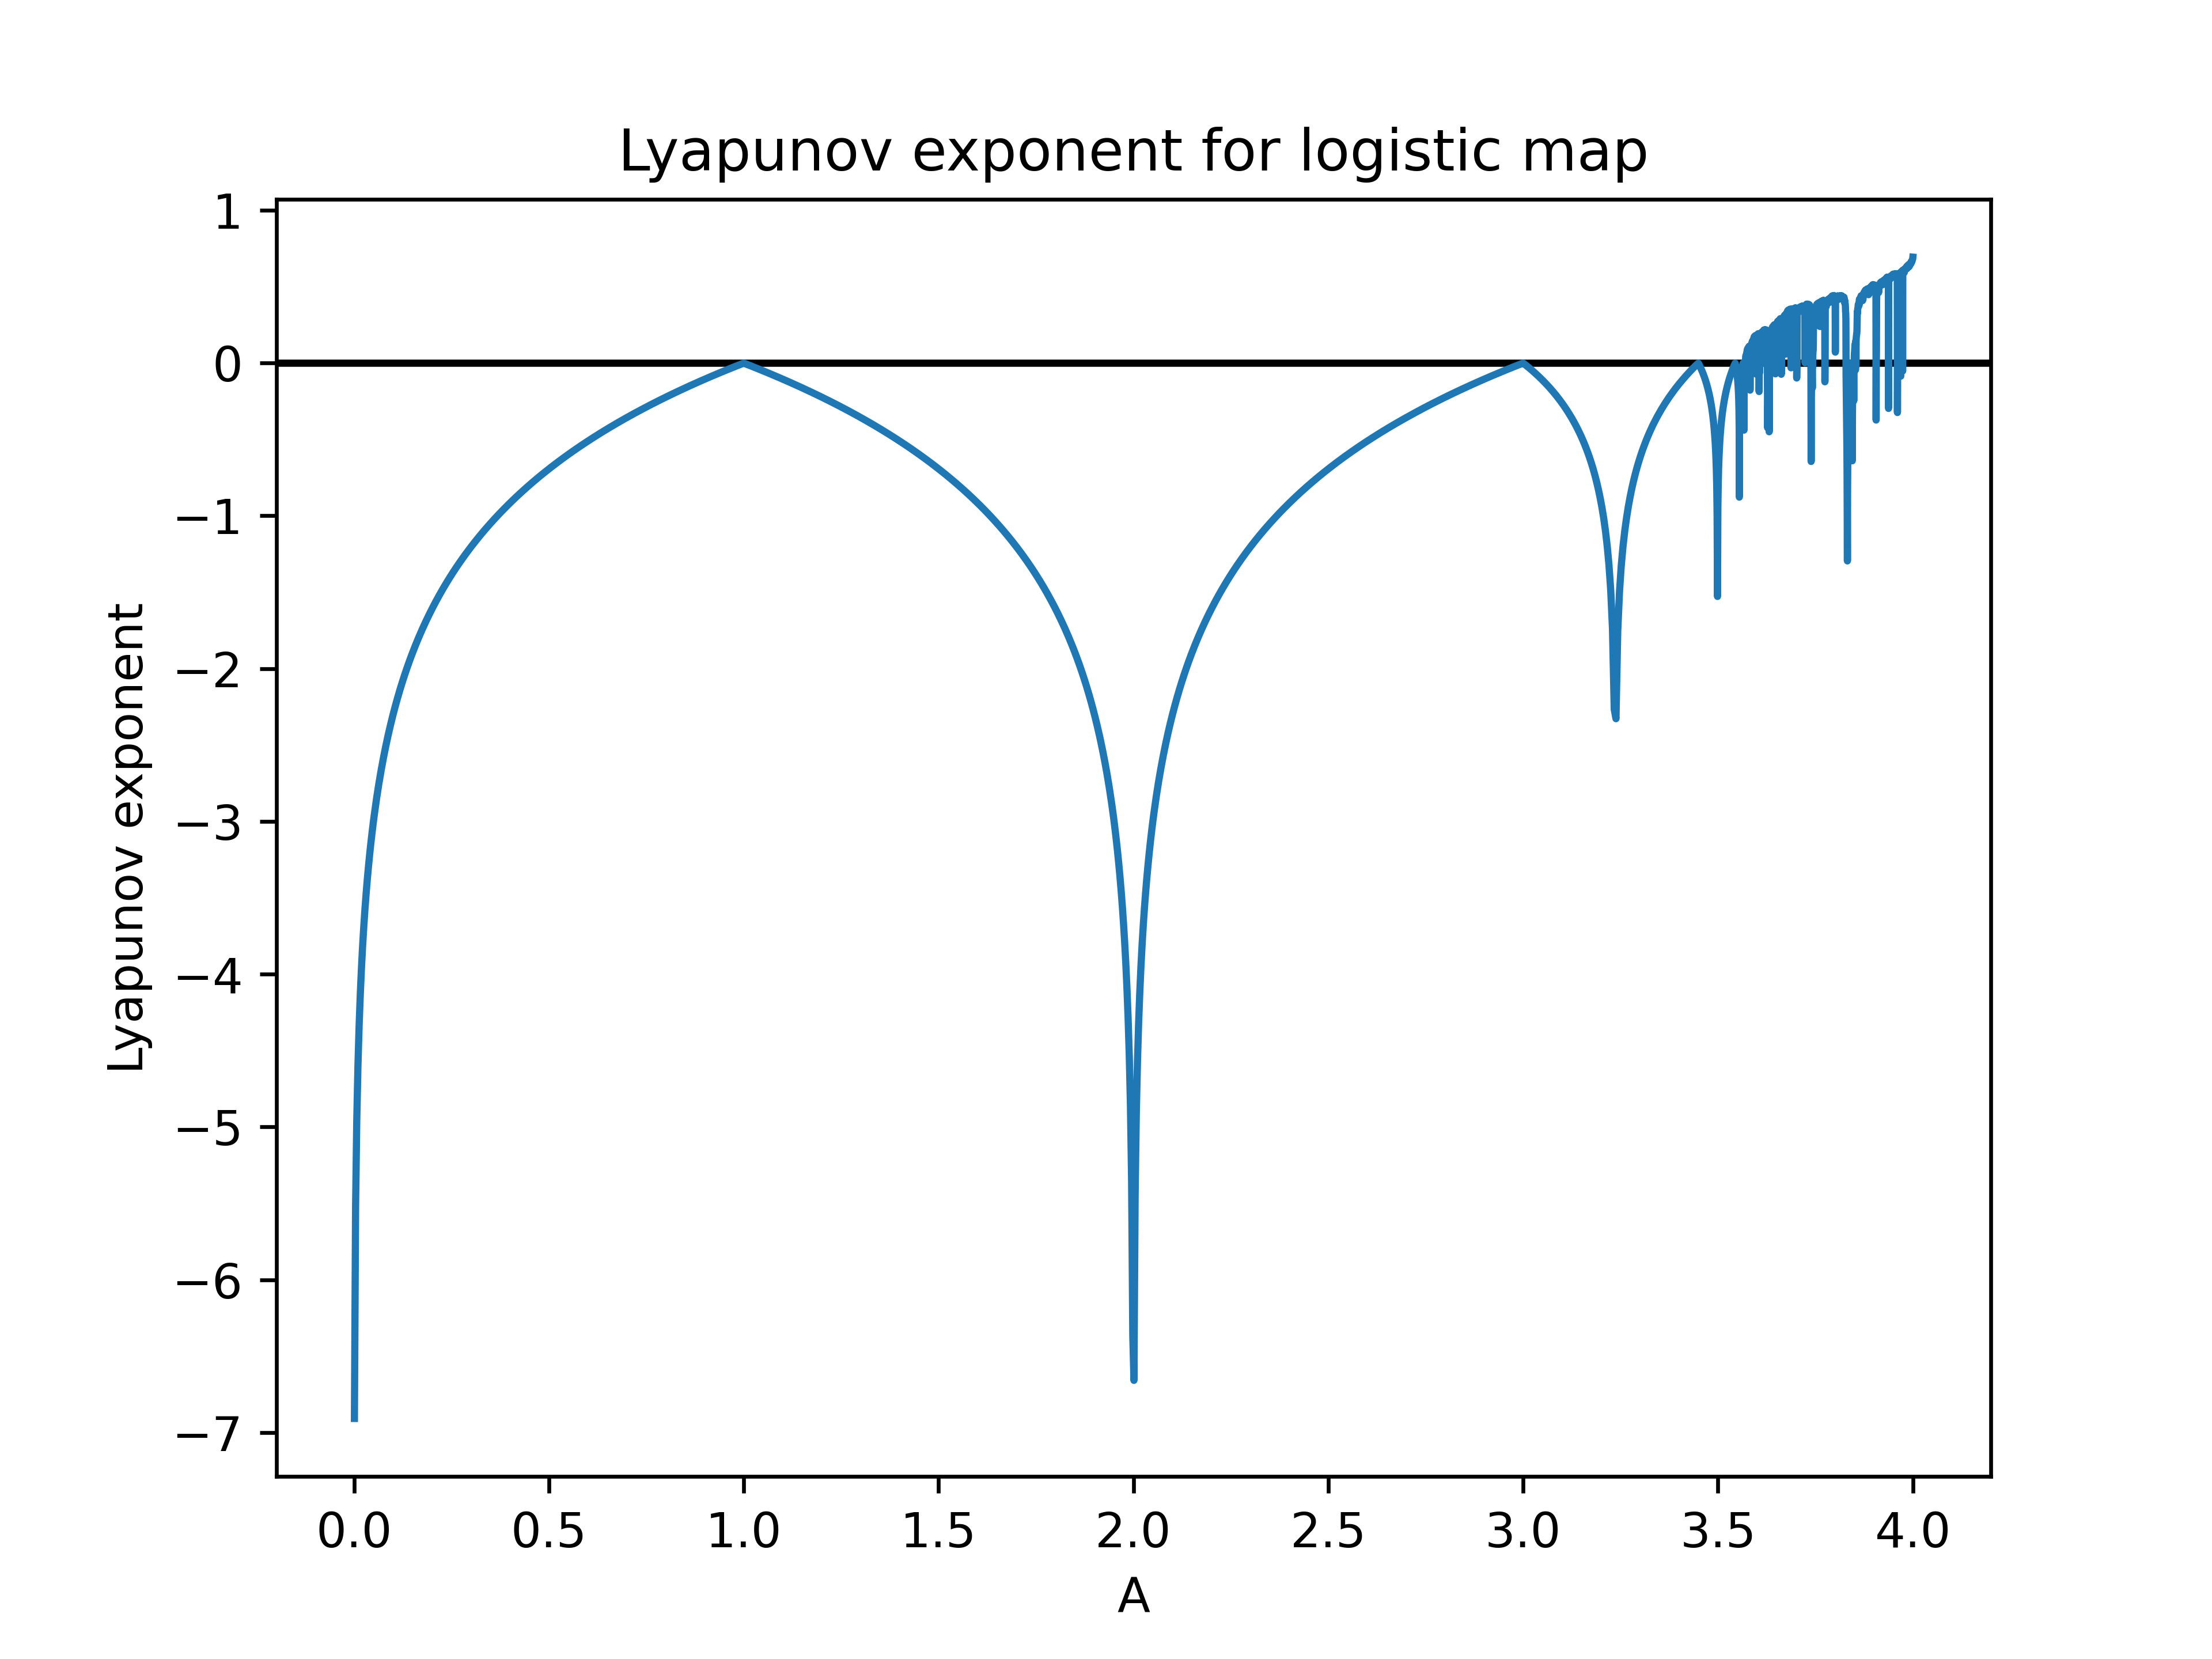
\includegraphics[width=0.6\linewidth]{logistic_lyapunov_exp.png}
    \end{figure}
\end{frame}

%------------------------------------------------

\section{Universality in One Dimensional Maps}
\subsection{Feigenbaum's Discovery}

\begin{frame}
	\frametitle{Feigenbaum's Discovery}
	
	\begin{itemize}
        \item While developing a quantitative description of period doubling in logistic map, Feigenbaum realised that precise functional form did not matter \pause
        \item Feigenbaum found out that a map on unit interval described by {\color{red}$F(x) = a\text{ }sin(\pi x)$} gave similar sequence of period doubling bifurcations \pause
    \end{itemize}

    \begin{figure}
		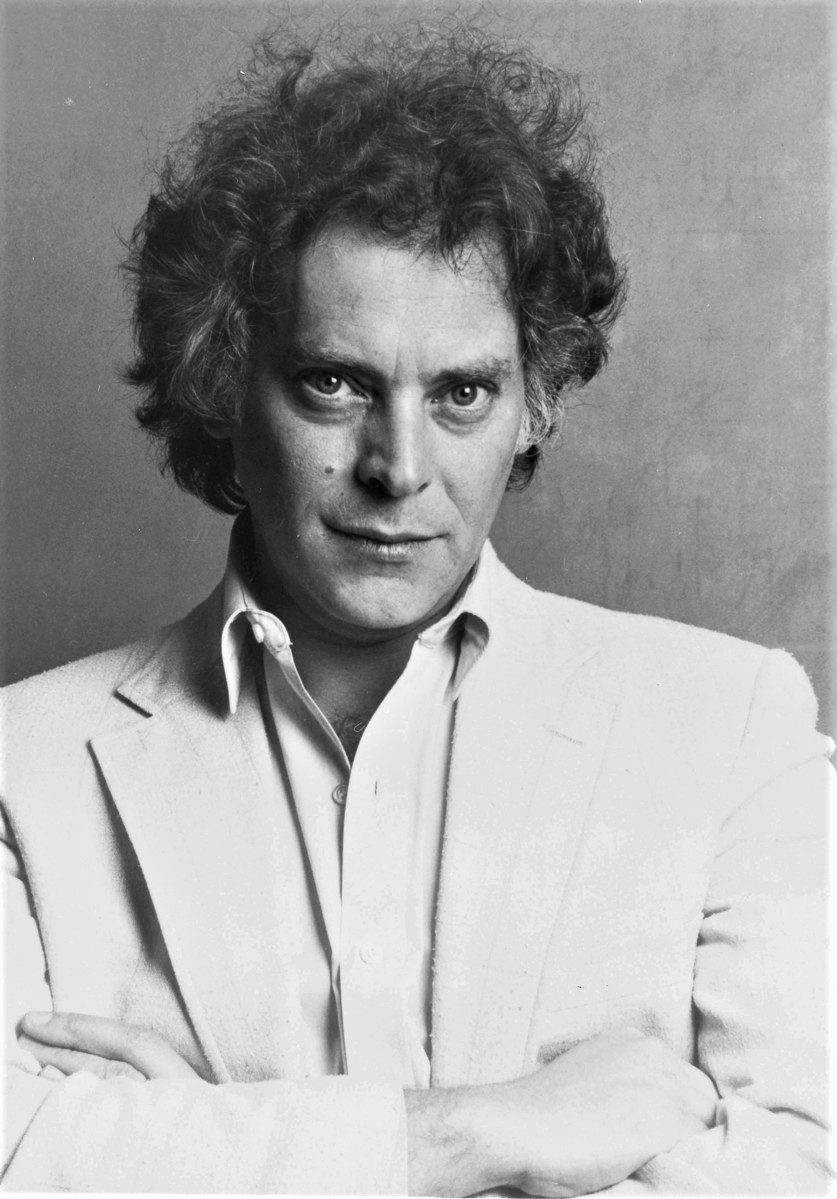
\includegraphics[width=0.15\linewidth]{feigenbaum.jpg}
		\caption{Mitchell Feigenbaum, 1987. Photo by Ingbert Grüttner}
	\end{figure}

\end{frame}

%------------------------------------------------

\begin{frame}
	\frametitle{Feigenbaum's Discovery}
	
	\begin{itemize}
        \item  Although the values of the control parameter a at which each period-doubling bifurcation occurs are different, he found that both the ratios of the changes in the control parameter and the separations of the stable daughter cycles decreased at the same geometrical rates $\delta$ and $\alpha$ as the logistic map. \pause
        \item This observation ultimately led to a rigorous proof, using the mathematical methods of the renormalization group borrowed from the theory of critical phenomena, that these geometrical ratios were universal numbers that would apply to the quantitative description of any period-doubling sequence generated by nonlinear maps with a single quadratic extremum. \pause
        \item The logistic map and the sine map are just two examples of this large universality class. The great significance of this result is that the global details of the dynamical system do not matter.
    \end{itemize}

\end{frame}

%------------------------------------------------

\begin{frame}
	\frametitle{Feigenbaum's Discovery}
	
	\begin{itemize}
        \item A thorough understanding of the simple logistic map is sufficient for describing both qualitatively and, to a large extent, quantitatively the period-doubling route to chaos in a wide variety of nonlinear dynamical systems. \pause
        \item In fact, this universality class extends beyond one-dimensional maps to nonlinear dynamical systems described by more realistic physical models corresponding to two-dimensional maps, systems of ordinary differential equations, and even partial differential equations.
    \end{itemize}

\end{frame}

%------------------------------------------------

\begin{frame}
	\frametitle{Overview}

    We will look at three different one dimensional maps: \pause

    \begin{itemize}
        \item Logistic Map \pause
        \item Sine Map \pause
        \item Quadratic Map
    \end{itemize}

\end{frame}

%------------------------------------------------

\subsection{Logistic Map}

\begin{frame}
	\frametitle{Logistic Map: Background}
    
        \begin{itemize}
            \item The logistic map is a polynomial mapping (equivalently, recurrence relation) of degree 2, often cited as an archetypal example of how complex, chaotic behaviour can arise from very simple non-linear dynamical equations. \pause
            \item The map was popularized in a seminal 1976 paper by the biologist Robert May, in part as a discrete-time demographic model analogous to the logistic equation first created by Pierre François Verhulst. \pause
            \item The logistic map is written
            \begin{equation}
                x_{n+1} = Ax_n(1-x_n)
            \end{equation}
            where $x_n$ denotes the ratio of existing population to the maximum possible population at discrete time $n$, and $A$ denotes a parameter measuring the rate of growth.
        \end{itemize}

\end{frame}

%------------------------------------------------

\end{document} 